% Chapter 2

\chapter{Gaussian processes} % Main chapter title

\label{Chapter2} % For referencing the chapter elsewhere, use \ref{Chapter2} 

%----------------------------------------------------------------------------------------

In Chapter \ref{Chapter1} we introduced the problem and the Bayesian optimization approach to solving it, using Gaussian processes (GPs) as emulators. In this chapter we will discuss the GP and show how it may be used to model the objective function $f$.

Intuitively, GPs are a generalization of the multivariate Gaussian distribution to infinite dimension. As such, GPs inherit many helpful properties from the multivariate Gaussian, which we review here. 

\section{Multivariate Gaussian distribution}

The random vector $\x = (x_1,...,x_d)^T \in \mathbb{R}^d$ has multivariate Gaussian distribution with mean vector $\B{m}$ and covariance matrix $\Sigma$ if its probability density is given by:
%
\begin{equation} \label{eq:gaussian}
f(\x) = \frac{1}{(2\pi)^{q/2}{\left | \Sigma  \right |}^{1/2}} \textrm{exp}\{{-\frac{1}{2}(\x-\B{m})^T \Sigma^{-1} (\x-\B{m})}\}
\end{equation}
%
This is denoted by $\x \sim \N(\B{m}, \Sigma)$ \cite{sm3}. 

The following (non-trivial) closure properties \citep{krzanowski} of the multivariate Gaussian make it particularly convenient for modelling:

\begin{enumerate}[label={G}{\arabic*}]
\item{ \label{itm:g1}
Marginal distributions of any subset of $\x$ are multivariate Gaussian. Consider partitioning $\x$ into $[\x_1, \x_2]$ where $\x_1 \in \mathbb{R}^p$ and $\x_2 \in \mathbb{R}^q$ with $p + q = d$, so that
%
\begin{equation}
\x = \colvec{2}{\x_1}{\x_2} \sim 
\N\left(\colvec{2}{\B{m}_1}{\B{m}_2}, 
\begin{bmatrix} \Sigma_{11} & \Sigma_{12} \\ \Sigma_{21} & \Sigma_{22} \end{bmatrix}\right) 
\end{equation}
%
where $\B{m}$ and $\Sigma$ are partitioned naturally. Then the marginal distribution of $\x_1$ is:
%
\begin{equation}
p(\x_1) = \N(\x_1 \vert \B{m}_1, \Sigma_{11})
\end{equation}
}
\item{ \label{itm:g2} 
Similarly, the conditional distribution of any subset of $\x$ conditioned another subset is multivariate Gaussian. The distribution of $\x_1$ given that $\x_2$ is known is given by:
%
\begin{equation}
p(\x_1 \vert \x_2) = 
\N(\x_1 \vert \B{m}_1 + \Sigma_{12}\Sigma_{22}^{-1}(\x_2 - \B{m}_2),
\Sigma_{11} - \Sigma_{12}\Sigma_{22}^{-1}\Sigma_{21})
\end{equation}
}
\end{enumerate}

\section{Gaussian process definition}

A \textit{Gaussian process} is defined to be a collection of random variables, any finite number of which have a joint Gaussian distribution \cite{rasmussen}. The random variables $f(\x)$ are indexed by the elements $\x$ of some set $\D$. 

As we have seen, the multivariate Gaussian distribution defined by equation \ref{eq:gaussian} is specified entirely by its mean vector $\B{m}$ and covariance matrix $\Sigma$. Analogously, a GP is specified entirely by its prior mean function $\mu_0:\D \to \mathbb{R}$ and covariance function $k:\D^2 \to \mathbb{R}$, with:
%
\begin{align}
\mu_0(\x) &= \mathbb{E}[f(\x)] \\
k(\x, \x') &= \Cov(f(\x), f(\x'))
\end{align}
%
This is commonly written as:
%
\begin{equation}
f(\mathbf{x}) \sim \mathcal{GP}(\mu_0(\mathbf{x}), k(\mathbf{x}, \mathbf{x'}))
\end{equation}

GPs are an example of the broader category of continuous stochastic processes, which may be intuitively thought of as random functions. For this reason GPs can be used as priors and posteriors over functions. This makes them a natural tool for sequential, Bayesian learning.

As we will be using GPs to model the objective function $f$ with domain $\D \subseteq \mathbb{R}^d$ we also assume that the index set is a compact subset of $\mathbb{R}^d$, although this is not a necessary assumption in the wider context.

\section{Kernel functions}

The covariance function $k$ is also regularly called the \textit{kernel} function. It is a positive-definite measure of the expected similarity of two inputs in the output space. 

The structure of a GP is primarily determined by the kernel as it specifies the likely properties of functions drawn from the process \cite{snelson2008flexible}. It is frequently assumed that the prior mean function is a constant, both for convenience and because uncertainty about the mean function can be encapsulated by the kernel \cite{duvenaud2014automatic}. In practise, this constant may be inferred from the data \cite{lizotte} as a part of model selection. However for simplicity, in this project we will take it to be zero. 

For these reasons, the choice of an appropriate kernel for the problem at hand is crucial. Similarly to the choice of an uninformative prior distribution for Bayesian inference about a parameter for which little is known, for Bayesian optimization it is reasonable to choose a kernel function which is flexible and does not impose strong assumptions. Two of the most widely used kernels, in part because of their suitability to this purpose, are the squared exponential kernel and members of the Matérn family of kernels.

\subsection{Squared exponential} \label{sec:sekernel}

The \textit{squared exponential} (SE) kernel produces sample functions that are infinitely differentiable, and so can be used to model functions which are very smooth.
%
\begin{equation}
k_{\mathrm{SE}}(\x, \x') = \sigma_f^2\:\mathrm{exp}\left(\frac{- \lvert \x - \x' \rvert ^2}{2l^2}\right)
\end{equation}
%
Variables which are close in the input space are highly correlated, the correlation decreasing as variables become further apart. The kernel attains a maximum value of $\sigma_f^2$ at $(\x, \x)$. 

The amplitude $\sigma_f^2$ and length-scale $l$ are examples of kernel \textit{hyper-parameters}, which in general we will denote by the vector $\param$. The amplitude controls the overall scale of variation. The length-scale controls how quickly the exponential decays and thus the rate at which input variables become de-correlated.

In general, kernel hyper-parameters substantially alter the behaviour of sample functions and generalisation properties of GP models. For this reason they should be tuned as a part of model selection, which will be detailed in section \ref{sec:modelselection}. 

Plots (a), (c) and (e) in figure \ref{fig:2i} show the effect of changing the length-scale $l$ on sample functions drawn from a GP with SE kernel: the smaller the value of $l$ the more wiggly the samples. In fact, this may be measured by the mean number of level-zero upcrossings on the unit-interval, which for a GP with SE kernel and mean-zero in one-dimension is $(2 \pi l)^{-1}$ \cite{rasmussen}. The effect of changing the amplitude $\sigma_f^2$ has not been shown in figure \ref{fig:2i}, as it simply corresponds to rescaling the y-axis.

\subsection{Matérn}

For realistic optimization problems the distribution of functions generated by squared exponential kernels may be unrealistically smooth \citep{snoek2012practical} \citep{stein2012interpolation}. An alternate suggestion is to use a member of the more general \textit{Matérn} family \citep{matern2013spatial}, which allows the smoothness to be controlled.
%
\begin{equation}
k_\mathrm{M}(\x, \x') = 
\frac{\sigma_f^2}{2^{\nu - 1}\Gamma(\varsigma)} \left(\frac{\sqrt{2\varsigma}\lvert \x - \x' \rvert}{l}\right)^\nu
K_\nu\left(\frac{\sqrt{2\nu}\lvert \x - \x' \rvert}{l}\right)
\end{equation}
%
Here $\sigma_f^2$ and $l$ are amplitude and length-scale as before, $\nu > 0$ is an additional hyper-parameter which controls how rough the sample functions are, $K_\nu$ is a modified Bessel function of the second kind and $\Gamma(\cdot)$ is the Gamma function. 

Sample functions produced by the Matérn kernel are $\left\lfloor{\nu}\right\rfloor$ times differentiable \citep{santner2013design}. In the limit as $\nu \to \infty$ the squared exponential kernel is recovered. 

Plots (b), (d) and (f) in figure \ref{fig:2i} show sample functions drawn from a GP with Matérn kernel, with $\nu = 1/2, 3/2$ and $5/2$. These particular values of $\nu$ are chosen as when $\nu = p + 1/2$ for some $p \in \mathbb{N}$ then the Matérn kernel may be simply expressed as the product of an exponential and a polynomial of order $p$ \cite{rasmussen}. Although it may be argued that the roughness should be learned from the data \cite{stein2012interpolation} it is common to chose $\nu$ to be either $3/2$ or $5/2$ outright \cite{lectures}, for which:
%
\begin{align}
k_\mathrm{M3/2}(\x, \x') &= \left(1 + \frac{\sqrt{3}\lvert \x - \x' \rvert}{l}\right) \mathrm{exp}\left(-\frac{\sqrt{3}\lvert \x - \x' \rvert}{l}\right) \\
k_\mathrm{M5/2}(\x, \x') &= \left(1 + \frac{\sqrt{5}\lvert \x - \x' \rvert}{l} + \frac{5\lvert \x - \x' \rvert^2}{3l^2}\right)\mathrm{exp}\left(-\frac{\sqrt{5}\lvert \x - \x' \rvert}{l}\right)
\end{align}

\begin{figure}
\centering
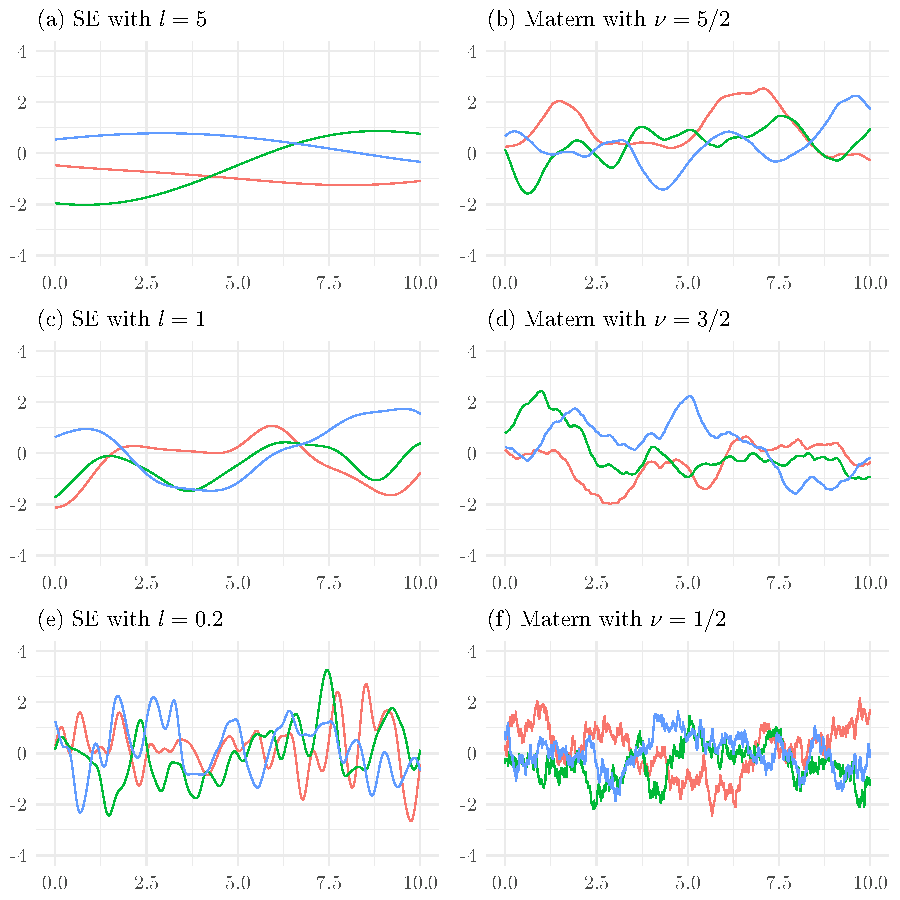
\includegraphics[scale=0.9]{fig2i.pdf}
\caption{Six plots, each with three samples from a zero-mean GP. Amplitude is $\sigma_f^2 = 1$ for each plot. In the plots (b), (d) and (f) with Matérn kernel, the length-scale $l = 1$. Variation in the length-scale of the Matérn kernel would have the same effect as in the squared exponential kernel, which is shown in plots (a), (c) and (e).} \label{fig:2i}
\end{figure}

\subsection{Automatic relevance determination}

Both of the above squared exponential and Matérn kernels are called \textit{stationary} as they are functions of $x - x'$. This means that they are invariant to transformations in the input space and corresponds to the modelling assumption that the objective function varies uniformly across the domain.

Further, since they are also both functions of $\lvert \x - \x' \rvert$ they are called \textit{isotropic} - uniform in all directions. However, this is often not the case and it would be advantageous to allow the kernel to express different rates of variation in different dimensions. More general \textit{anisotropic} kernels may be defined by replacing $\lvert \x - \x' \rvert^2$ by
%
\begin{equation}
r^2(\x, \x') = (\x - \x')^T D (\x - \x')
\end{equation}
%
for some positive semi-definite matrix $D$. Of course if $D$ is a dense (non-sparse) matrix it introduces many hyper-parameters, which may be difficult to deal with. As such, a popular choice for $D$ is a diagonal matrix with entries $D_{j,j} = 1/l_j^2$ such that:
%
\begin{equation}
r^2(\x, \x') = \sum_{j=1}^{d} \frac{(x_j - x'_j)^2}{l_j^2} \label{ard}
\end{equation}
%
The $l_j$ are simply individual length-scale hyper-parameters for each dimension. Kernels which are functions of equation \ref{ard} are called \textit{automatic relevance determination} kernels \cite{neal1996bayesian} as they allow for the relative importance of each dimension to be learned when the kernel hyper-parameters are tuned. This is helpful in dealing with cases where the objective function has low effective dimensionality, as was briefly mentioned in section \ref{sampledesigns}.

\section{Sampling from a Gaussian process}

Consider that we are interested in sampling from a zero-mean GP at a finite collection of points $\x_{1:n} := \{\x_1, \ldots, \x_n\}$, where each $\x$ is in $\D$. Since each $\x$ is itself a vector, any finite vector of indices induces a matrix which we denote by $X := [\x_1, \ldots , \x_n]^T \in \D^n \subseteq \mathbb{R}^{n \times d}$. The vector of random variables $\f := f(X) := [f(\x_1), \ldots , f(\x_n)]^T$ corresponding to this matrix by definition has a joint multivariate Gaussian distribution.

The parameters of this distribution are determined by applying the mean and kernel functions: $\f$ has mean vector $\B{0}$ and covariance matrix $K := k(X,X)$ with elements $K_{i,j} = k(\x_i,\x_j), \forall i=1, \ldots, n, j=1, \ldots, n$. The requirement that the kernel $k$ is positive-definite precisely means that any such matrix $K$, sometimes called the Gram matrix, is a valid covariance matrix. So, the distribution of $\f$ is:
%
\begin{equation}
\colvec{4}{f(\x_1)}{f(\x_2)}{\vdots}{f(\x_n)} \sim \N \left(
\colvec{4}{0}{0}{\vdots}{0}, 
\begin{bmatrix} k(\x_1, \x_1) & k(\x_1, \x_2) & \ldots & k(\x_1, \x_n) \\ 
				k(\x_2, \x_1) & k(\x_2, \x_2) & \ldots & k(\x_2, \x_n) \\
				\vdots        & \vdots        & \ddots & \vdots        \\
				k(\x_n, \x_1) & k(\x_n, \x_2) & \ldots & k(\x_n, \x_n) \\ 
\end{bmatrix}
\right)
\end{equation}
%
Put more succinctly:
\begin{equation}
\f \sim \N(\B{0}, K) \label{eq:ml}
\end{equation}
%
This distribution is referred to as the marginal likelihood, as it implicitly marginalizes out all possible function values at every $\x \in \D$ which is not in $\x_{1:n}$ \cite{duvenaud2014automatic}. This is justified by property \ref{itm:g1} of the multivariate Gaussian. For this reason, although a GP is an infinite object it is only ever necessary to consider finite subsets. Discretizing the domain and using equation \ref{eq:ml} allows us to visualize samples from a GP, as in figure \ref{fig:2i}.

Although this all does not seem particularly useful as it stands, shortly we will show that this distribution may be used as a prior in order to perform inference directly in function-space. It is for this reason that the notation $\mu_0$ is chosen for the prior mean function. First, however, we will take a brief interlude to discuss Bayesian linear regression and how it relates to GPs.

\section{Bayesian linear regression} 

Given a training data-set of observations and a new vector $\x_* \in \mathbb{R}^d$ of input variables, the aim of \textit{regression} is to predict target variable $f(\x_*)$. This is described as a \textit{supervised learning} task as the training data-set, i.e. the values of the target variable at the collection of inputs $\x_{1:n}$, plays the role of teaching us about the behaviour of $f$ \cite{sm3}. 

The approach of linear regression is to define a model in terms of a linear combination of fixed basis functions:
%
\begin{equation}
f(\x) = \B{w}^T\phi(\x)
\end{equation}
%
where $\B{w}^T$ is a vector of weights and $\phi(\x)$ is a vector of $M$ fixed non-linear basis functions that depend on the input vector $\x$. Many choices of basis functions are possible such as polynomial, Gaussian, sigmoidal or Fourier \cite{christopher2006pattern}. 

Typically the values of $\B{w}$ are estimated by minimizing the sum of squares error from the fitted values to the training data, which corresponds to finding the maximum likelihood estimator. This has analytic solution $\hat{\B{w}}$ given by the normal equations \cite{christopher2006pattern}
%
\begin{equation}
\hat{\B{w}} = \left(\B{\Phi}^T\B{\Phi}\right)^{-1}\B{\Phi}^T\f
\end{equation}
% 
where $\B{\Phi}$ is the design matrix with elements $\Phi_{n, k} = \phi_k(x_n)$ such that:
%
\begin{equation}
\B{\Phi} = 
\begin{pmatrix}
 \phi_1(\B{x}_1) & \phi_2(\B{x}_1) & \cdots & \phi_M(\B{x}_1) \\
 \phi_1(\B{x}_2) & \phi_2(\B{x}_2) & \cdots & \phi_M(\B{x}_2) \\
 \vdots  & \vdots  & \ddots & \vdots  \\
 \phi_1(\B{x}_n) & \phi_2(\B{x}_n) & \cdots & \phi_M(\B{x}_n) 
\end{pmatrix}
\end{equation}
%

A more Bayesian approach to this problem would be to place a prior distribution, say a Gaussian, on the weights $\B{w}$ such that:
%
\begin{equation}
p(\B{w}) = \N(\B{w} | \B{0}, \B{\Sigma}_w)
\end{equation}
%
where $\B{\Sigma}_w$ is the $M$ by $M$ covariance matrix. Notice that fixing $\B{w}$ fixes $f(\x)$, thus the probability distribution over $\B{w}$ induces a probability distribution over functions $f(\x)$. This distribution over functions is exactly a GP prior. As $f(\x)$ is a linear combination of Gaussian distributions it is itself Gaussian. The mean function $\mu_0$ is zero, as
%
\begin{align}
\nonumber \mu_0(\x) &= \E[f(\x)]  \\
\nonumber           &= \phi(\x) \E[\B{w}] \\
                    &= 0
\end{align}
%
and the covariance function is given by
%
\begin{align}
\nonumber k(\x, \x') &= \Cov(f(\x), f(\x')) \\
\nonumber            &= \E[f(\x)f(\x')] \\
\nonumber		     &= \phi(\x)^T \E[\B{w}^T\B{w}] \phi(\x') \\
		             &= \phi(\x)^T \Sigma_w \phi(\x')
\end{align}

This GP is called \textit{degenerate} precisely because it can be represented with a finite collection of basis functions as we have shown above. In fact, by Mercer's theorem, for every valid kernel function there exists a (possibly infinite) expansion in terms of basis functions \cite{rasmussen}. For example, taking $l^2 = \sigma_f^2 = 1$, the squared exponential kernel in one-dimension is given by \cite{vafa2016training}
%
\begin{align}
\nonumber k(x, x') = e^{- \frac{(x - x')^2}{2}} &= e^{-\frac{x^2}{2}}e^{-\frac{x'^2}{2}}\sum_{k=0}^{\infty} \frac{(xx')^k}{k!} \\
&= \phi(x)^T \phi(x')
\end{align}
where we have the infinite basis expansion
\begin{equation}
\phi(x) = e^{- \frac{(x - x')^2}{2}}\left[ 1, x, \frac{x^2}{\sqrt{2}}, \frac{x^3}{\sqrt{6}},... \right]
\end{equation}

\section{Gaussian process regression}

In this section we will show how regression can be done directly with GPs, \textit{without} having to think about the basis functions.

Suppose that at inputs $\x_{1:n}$ the values of the GP $\f = [f(\x_1), \ldots , f(\x_n)]^T$ are observed. We are interested in the value of the GP $f_* := f(\x_*)$ at a new input $\x_*$. By the GP definition, the joint prior distribution of $\f$ and $f_*$ is
%
\begin{equation} \label{eq:joint}
\colvec{2}{\f}{f_*} \sim \N \left(
\colvec{2}{\B{0}}{0},
\begin{bmatrix} K & k(X,\x_*)^T \\ 
				k(X,\x_*) & k(\x_*,\x_*) \\
\end{bmatrix} \right)
\end{equation}
%
where $k(X,\x_*) = [k(\x_1, \x_*), \ldots, k(\x_n, \x_*)]^T$ is the vector of covariance terms between the locations $\x_{1:n}$ and $\x_*$. For brevity this will in future be denoted by $\B{k}_*$. Now we make use of property \ref{itm:g2} of the multivariate Gaussian to find that the conditional distribution of $f_*$ given $\f$ is Gaussian
%
\begin{equation}
f_* \vert \f \sim \N(\mu_n(\x_*), \sigma^2_n(\x_*))
\end{equation}
%
with mean and variance given by
%
\begin{align} 
\mu_n(\x_*) &= \B{k}_*^T K^{-1} \f \label{eq:predmean} \\ 
\sigma^2_n(\x_*) &= k(\x_*,\x_*) - \B{k}_*^T K^{-1} \B{k}_* \label{eq:predvar}
\end{align}
%
This is known as the \textit{predictive distribution} as it gives the mean and variance at any given unobserved test point $\x_*$. 

Often, it is not possible to directly observe $\f$ itself.  Instead, we may observe a noise contaminated version $\y$, where each $y = f(\x) + \epsilon$ as in property \ref{itm:p4}. We assume Gaussian additive independent identically distributed noise with zero mean and variance $\sigma^2$ such that:
\begin{equation}
p(\y \vert \f) = \N(\y \vert \f, \sigma^2I)
\end{equation}
%
Integrating out the unobserved values $\f$ with distribution $p(\f)$ from equation \ref{eq:ml}, the marginal likelihood is:
%
\begin{align} \label{eq:mln}
p(\y) &= \int d\f \, p(\y|\f)p(\f) \\
      &= \N(\y \vert \B{0}, K + \sigma^2I) 
\end{align}
%
Introducing the additional noise term to \ref{eq:joint}, the joint distribution of the values $\y$ and $f_*$ is:
%
\begin{equation}
\colvec{2}{\y}{f_*} \sim \N \left(
\colvec{2}{\B{0}}{0},
\begin{bmatrix} K + \sigma^2I & \B{k}_*^T \\ 
				\B{k}_* & k(\x_*,\x_*) \\
\end{bmatrix} \right)
\end{equation}
%
This can be conditioned as before to show that the predictive distribution $p(\f_* \vert \y)$ is Gaussian with mean and variance given by:
%
\begin{align} \label{eq:npredmean}
\mu_n(\x_*) &= \B{k}_*^T(K + \sigma^2I)^{-1}\y \\
\sigma^2_n(\x_*) &= k(\x_*,\x_*) - \B{k}_*^T(K + \sigma^2I)^{-1}\B{k}_* \label{eq:npredvar}
\end{align}
%
Taking $\sigma^2 = 0$ recovers equations \ref{eq:predmean} and \ref{eq:predvar}. The predictive distribution actually defines a posterior Gaussian process in its own right \cite{snelson2008flexible} with mean function as in equation \ref{eq:npredmean} and kernel function
%
\begin{equation}
k(\x, \x') = k(\x,\x') - \B{k}^T(K + \sigma^2I)^{-1}\B{k}'
\end{equation}
%
where $\B{k} = [k(\x_1, \x), \ldots, k(\x_n, \x)]^T$ and $\B{k}'$ is defined similarly.

Observe that rather than depending on a fixed number of parameters, the complexity of the model adapts to the number of training data points \citep{orbanz2011bayesian}. As such, GP regression is an example of a Bayesian \textit{non-parametric} model, where the parameter-space is infinite. This is advantageous as we do not have to specify a parametric structure and have less worries about over-fitting, which in parametric modelling typically must be combated with regularization.

In equation \ref{eq:predmean} notice that that predictive mean is simply a linear combination of the of the observations. For this reason equation \ref{eq:predmean} is known as a linear predictor \cite{rasmussen} - in fact it is actually the best linear unbiased predictor \cite{lectures}.

In equation \ref{eq:npredvar} the predictive variance is the prior variance minus a (positive) term which only depends on the training data locations. The closer the training data locations $\x_{1:n}$ are to $\x_*$ the greater the values in the vector $\B{k}_*$ are, and the greater the Mahalanobis distance $\B{k}_*^T(K + \sigma^2I)^{-1}\B{k}_*$. This explains the visual effect, which can be seen in figure \ref{fig:2i}, of the predictive variance decreasing closer to the training data points. That being said, it may be considered disappointing that the predictive variance is completely independent of the actual values observed $\y$: surely if an unexpected value is observed then this should be accounted for by increased uncertainty. \citet{shah2014student} for this and other reasons propose the use of the more general Student-t process as an alternative to the GP.

\begin{figure}
\centering
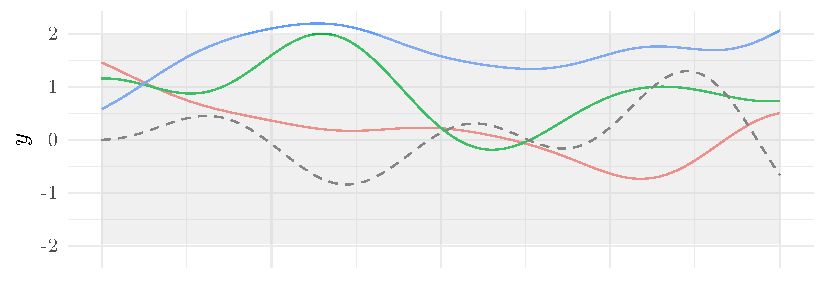
\includegraphics[scale=1]{fig2iia.pdf}
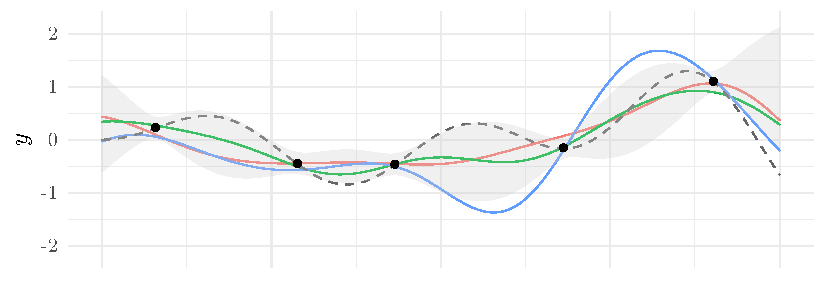
\includegraphics[scale=1]{fig2iib.pdf}
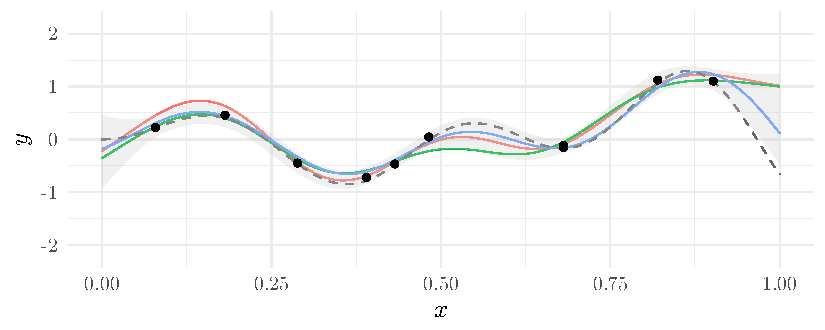
\includegraphics[scale=1]{fig2iic.pdf}
\caption{GP regression example. In each plot there are three samples curves from a GP with with prior mean zero and  squared exponential kernel with hyper-parameters $\param = (\sigma_f, l) = (1, 0.15)$. Data is generated by objective function $f(x) = \sin(5x)\sin(13x)\exp(x-0.5)$, shown as the grey dotted line, with additive Gaussian noise with variance $\sigma^2 = 0.01$. The shaded region is a $95\%$ confidence interval calculated using the predictive mean \ref{eq:npredmean} and variance \ref{eq:npredvar} equations.} \label{fig2ii}
\end{figure}

The dimension of the matrix $K$ is the number of data points observed $n$. This matrix is inverted in equations \ref{eq:predmean} and \ref{eq:predvar} usually by computing the Cholesky decomposition. This has computational cost big $\mathcal{O}(n^3)$, which is typically the bottleneck of GP regression - limiting it's reach to relatively small $n$. This has motivated the development of sparse Gaussian processes \cite{quinonero2005unifying} \cite{snelson2006sparse} which approximate the posterior over functions to make inference computationally cheaper.

\section{Learning the hyper-parameters} \label{sec:modelselection}

In the complete hierarchical Bayesian model selection framework \cite{mackay1992bayesian} models are specified in three tiers: model parameters, model hyper-parameters and model structures. We will focus our attention on model selection at the second level, the model hyper-parameters.

At the bottom level the model parameters are obtained by the posterior distribution over functions, as our model is non-parametric. The top level corresponds to the choice of kernel function, which is one of the key challenges of GP regression. To alleviate potential problems, the kernel functions chosen are purposefully flexible as we have discussed. 

This leaves the model hyper-parameters, which are the hyper-parameters of the kernel function $\param$ together with the noise-variance $\sigma^2$ if it is unknown. The most simplistic approach would be to specify the hyper-parameters a-priori, however ill-fitting choices, illustrated in figure \ref{fig:2iii}, can lead to very poor performance. As a result it is better to learn the hyper-parameters from the data, which may be done by maximizing the marginal likelihood, which is analytic for GP models and given by equation \ref{eq:mln}. Making the dependence of $K$ on the kernel hyper-parameters $\param$ explicit, its logarithm is:
%
\begin{align} \label{eq:loglike}
\nonumber \log p(\y \vert X, \param) = 
&-\frac{n}{2}\log2\pi 
\underbrace{-\frac{1}{2}\log\lvert K_{\param} + \sigma^2I \rvert}_{\text{controls model capacity}} \\
& \underbrace{- \frac{1}{2} \y^T(K_{\param} + \sigma^2I)^{-1}\y}_{\text{encourages fit with data}}
\end{align}
%
Optimizing this likelihood gives an empirical Bayes estimate for the hyper-parameters. Equation \ref{eq:loglike} balances the trade-off between fit and complexity of the model \cite{duvenaud2014automatic}. The second term penalizes the complexity of the model as the determinant of the covariance matrix grows with more complicated kernels, such as those with  smaller length-scales. The final term is a Mahalanobis distance which controls the quality of the fit.

\begin{figure}
\centering
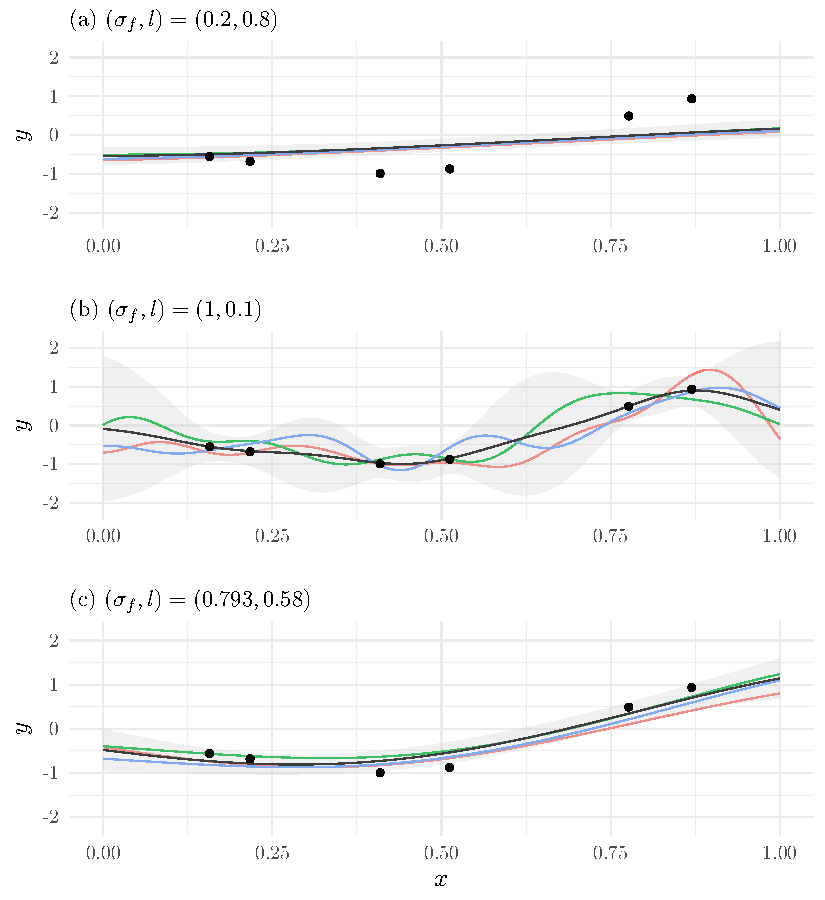
\includegraphics[scale=1]{fig2iii.pdf}
\caption{The impact of different amplitude and length-scale hyper-parameters on squared exponential kernel GP regression models. As in figure \ref{fig2ii} there are three sample curves with the addition of a black mean function. Figure (a) is an example of under-fitting the data. It is overly simplistic and fails to capture the underlying trend in the data. Figure (b) is an example of over-fitting. It is a more complex model which has mean function that interpolates the data. Finally, figure (c) uses the maximum likelihood estimates of the hyper-parameters and is a balance between figures (a) and (b).} \label{fig:2iii}
\end{figure}

There are many possible ways to optimize equation \ref{eq:loglike}. One alternative is to use quasi-Newton methods such as the Broyden–Fletcher–Goldfarb–Shanno (BFGS) algorithm with random restarts. In this project we will use the L-BFGS-B algorithm \cite{byrd1995limited} which approximates the BFGS algorithm and is adapted to handle simple box-constraints on the hyper-parameters, i.e. bounded above and below. This algorithm is used in many R implementations of GP regression such as the \texttt{DiceKriging} \cite{roustant2012dicekriging}, \texttt{GPfit} \cite{macdonald2013gpfit} and \texttt{laGP} \cite{gramacy2016lagp} packages.

In Bayesian optimization, the hyper-parameters are typically tuned at every iteration of the algorithm - in particular whenever a GP is fit.